\documentclass[12pt,a4paper]{article}
\usepackage{geometry}
\geometry{margin=2.5cm}
\usepackage{setspace}
\usepackage{graphicx}
% \usepackage{amsmath}
\usepackage{multirow}
\usepackage{caption}
\usepackage{booktabs}
\usepackage{float}
\usepackage{xcolor}
\usepackage{tcolorbox}
\usepackage{titlesec}
\usepackage{hyperref}

% Etc
\usepackage{titling}
% \usepackage{csquotes}

% math packages
\usepackage{enumitem}
\usepackage{amsmath,amssymb,amsthm}
\usepackage{algorithm}
\usepackage{algpseudocode}

\theoremstyle{remark}
\newtheorem*{solusi}{Solusi}

\setstretch{1.25}
\setlength{\parskip}{0.5em}
\setlength{\parindent}{0pt}

% \usepackage[indonesian]{babel}
\usepackage{csquotes}
\usepackage[
  backend=biber,
  style=ieee,
  language=auto,
  autolang=other
]{biblatex}

\DefineBibliographyStrings{english}{%
  references   = {Daftar Pustaka},
  bibliography = {Daftar Pustaka},
%   online       = {Daring},
  and          = {dan},
  andothers    = {dkk.},
  pages        = {hlm.},
  urlseen      = {diakses},
  % bulan:
  january      = {Januari},
  february     = {Februari},
  march        = {Maret},
  april        = {April},
  may          = {Mei},
  june         = {Juni},
  july         = {Juli},
  august       = {Agustus},
  september    = {September},
  october      = {Oktober},
  november     = {November},
  december     = {Desember},
%   available    = {tersedia},
}


% \DeclareLanguageMapping{indonesian}{indonesian}
\addbibresource{refs.bib}

% % times new roman
% \usepackage{newtxtext,newtxmath}

\renewcommand{\thesection}{\Alph{section}}
\renewcommand{\thesubsection}{\arabic{subsection}}
\renewcommand{\thesubsubsection}{\thesubsection.\arabic{subsubsection}}

% Format section menggunakan tcolorbox
\definecolor{headerbg}{RGB}{0,0,0}
\definecolor{headertext}{RGB}{255,255,255}


\newtcolorbox{sectionbox}{
  colback=headerbg,
  coltext=headertext,
  boxrule=0pt,
  arc=0pt,
  left=4pt,
  right=4pt,
  top=1pt,
  bottom=1pt,
  width=\dimexpr\textwidth\relax,
}

\titleformat{\section}[block]
  {\normalfont\bfseries}
  {}{0pt}
  {\begin{sectionbox}\thesection\ }[\end{sectionbox}]


% OVERRIDE Caption
\captionsetup[figure]{labelfont=bf, name=Gambar, justification=centering}
\captionsetup[table]{labelfont=bf, name=Tabel, justification=centering}

% --- Title page ---
\title{%
  \textbf{Tugas Mata Kuliah} \\
  \large Prinsip Kecerdasan Artifisial \\
  \large Tugas Opsional UTS}
  
\author{Khalilullah Al Faath \\ NIU: 566643 \\ Magister Ilmu Komputer \\ [1cm]
  
\includegraphics[width=0.4\textwidth]{images/logo-ugm.png}}
\date{Universitas Gadjah Mada \\ Semester Gasal 2025/2026}

\makeatletter
\renewcommand{\maketitle}{%
  \begin{titlepage}
    \centering
    \vspace*{2cm}
    
    {\LARGE \@title \par}
    \vspace{2cm}
    
    {\large \@author \par}
    
    \vfill
    
    {\large \@date \par}
  \end{titlepage}
}
\makeatother


\begin{document}

\maketitle
\thispagestyle{empty}


\begin{center}
    \Large \textbf{BAB}\\[1em]
    \large \textbf{LOGIKA FUZZY}\\[2em]
\end{center}

\section{Tujuan Penjelasan Bab}
Setelah mengikuti penjelasan bab ini, pembaca diharapkan dapat:
\begin{enumerate}
    \item Memahami konsep dasar logika fuzzy serta perbedaannya dengan logika biner klasik.
    \item Menjelaskan struktur sistem fuzzy yang terdiri dari proses fuzzifikasi, basis aturan, mesin inferensi, dan defuzzifikasi.
    \item Mengidentifikasi jenis-jenis fungsi keanggotaan dan penerapannya dalam pemodelan ketidakpastian.
    \item Mengimplementasikan sistem inferensi fuzzy sederhana (misalnya metode Mamdani atau Sugeno) melalui contoh kasus nyata.
    \item Mengevaluasi kelebihan dan keterbatasan logika fuzzy dibandingkan dengan pendekatan deterministik maupun probabilistik.
\end{enumerate}


\section{Pendahuluan}

Sistem logika klasik, seperti logika proposisi (\textit{propositional logic}) dan logika predikat tingkat pertama (\textit{first-order logic}), setiap pernyataannya hanya mengenal dua keadaan: benar (\textit{true}) atau salah (\textit{false}). Pendekatan biner seperti ini efektif untuk komputasi matematis dan digital,
tetapi sering kali tidak cukup fleksibel untuk merepresentasikan kompleksitas dunia nyata.
Dalam banyak kasus, fenomena nyata tidak sepenuhnya hitam atau putih,
melainkan memiliki tingkat keabuan di antaranya.

Untuk mengatasi keterbatasan tersebut, muncul \textbf{logika fuzzy}
sebagai metode yang memungkinkan nilai kebenaran berada di antara 0 dan 1. Logika fuzzy adalah sebuah bentuk logika banyak nilai (\textit{many-valued logic}) dengan nilai kebenaran tiap variabelnya bisa bernilai bilangan riil apapun dari 0 sampai 1 \cite{novak_mathematical_1999}.
Dengan logika fuzzy, konsep seperti “suhu panas”, “kecepatan sedang”,
atau “risiko rendah” dapat dimodelkan secara kuantitatif menggunakan
fungsi keanggotaan (\textit{membership function}).

Pendekatan ini pertama kali diperkenalkan oleh Lotfi A. Zadeh pada tahun 1965,
dan sejak itu telah menjadi dasar bagi berbagai sistem cerdas
seperti kontrol suhu otomatis, sistem pendukung keputusan, dan klasifikasi data
dalam bidang kecerdasan buatan \cite{fogarty_fuzzy_2021}.

\section{Konsep Utama}

Bagian ini membahas konsep dasar yang menjadi fondasi dari logika fuzzy, mulai dari pengertian nilai keanggotaan hingga proses penalaran dan pengambilan keputusan berbasis fuzzy.

% TODO: Masukkan definisi fuzzy set
% TODO: Masukkan definisi fuzzy logic

\subsection{Definisi dan Istilah Dasar}

Sebelum membahas lebih jauh mengenai prinsip kerja logika fuzzy, penting untuk memahami terlebih dahulu beberapa istilah dan notasi dasar yang digunakan dalam pembahasan ini. Istilah-istilah berikut akan menjadi fondasi bagi penjelasan konsep lanjutan seperti derajat keanggotaan, fungsi keanggotaan, dan proses inferensi fuzzy.

\subsubsection{Semesta Pembicaraan (\textit{Universe of Discourse})} \label{section:semesta_pembicaraan}
Semesta pembicaraan adalah ruang atau himpunan semua kemungkinan elemen yang relevan untuk masalah yang sedang dikaji \cite{ross_fuzzy_2016}. Contoh: jika masalahnya adalah klasifikasi suhu, maka semestanya bisa berupa semua nilai suhu yang mungkin (misalnya dari 0°C sampai 100°C).

\subsubsection{Himpunan (\textit{Set})}
Himpunan adalah kumpulan elemen atau objek yang memiliki karakteristik tertentu dan dapat didefinisikan dengan jelas. Dalam logika klasik, keanggotaan suatu elemen terhadap himpunan bersifat tegas (disebut juga \textit{Crisp Set} atau \textbf{Himpunan Tegas}), sedemikian sehingga elemen tersebut \textit{hanya bisa} menjadi anggota atau bukan anggota \cite{ross_fuzzy_2016}.
Sebagai contoh, jika didefinisikan himpunan tegas dalam semesta pembicaraan dalam Bagian \ref{section:semesta_pembicaraan},
\[
    A = \{x \mid 27 \leq x \leq 35\},
\]
yang merepresentasikan "suhu hangat' dalam derajat Celcius, maka elemen $x=30$ merupakan anggota dari $A$, sedangkan $x=25$ bukan anggota $A$.

Di sisi lain, himpunan fuzzy (himpunan kabur) adalah generalisasi dari himpunan klasik yang setiap elemennya tidak hanya dinyatakan sebagai anggota atau bukan anggota, tetapi memiliki tingkat keanggotaan tertentu terhadap himpunan tersebut. Secara matematis, himpunan fuzzy \(A\) didefinisikan sebagai:
\[
    A = \{(x, \mu_A(x)) \mid x \in X\}.
\]
Dengan demikian, \textbf{himpunan fuzzy} merupakan kumpulan pasangan nilai yang menunjukkan elemen \(x\) beserta derajat keanggotaannya terhadap \(A\). Misalnya, suhu 29°C bisa dianggap “hangat” dengan keanggotaan 0.7, sedangkan 25°C dengan 0.4. Gambar \ref{fig:crisp_and_fuzzy} menggambarkan perbedaan keduanya.

\begin{figure}[H]
    \centering
    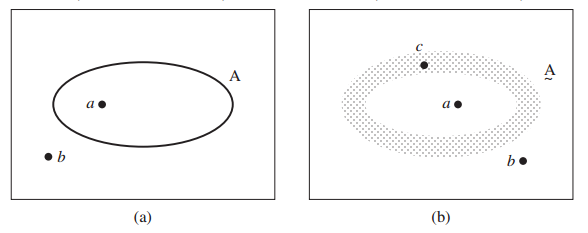
\includegraphics[width=1\linewidth]{images/fuzzy.png}
    \caption{Perbedaan antara (a) Himpunan Tegas dan (b) Himpunan Kabur \cite{ross_fuzzy_2016}}
    \label{fig:crisp_and_fuzzy}
\end{figure}



\subsubsection{Fungsi Keanggotaan (\textit{Membership Function})}
Fungsi keanggotaan merepresentasikan hubungan antara elemen pada semesta pembicaraan dan tingkat keanggotaannya terhadap suatu himpunan \cite{ross_fuzzy_2016}. Dalam logika klasik, fungsi ini disebut \textit{fungsi karakteristik} (\(\chi_A(x)\)) yang memetakan setiap elemen \(x \in X\) ke dua nilai diskrit, yaitu 0 atau 1:
\[
    \chi_A(x) =
    \begin{cases}
        1, & x \in A,    \\
        0, & x \notin A.
    \end{cases}
\]
Pemetaan ini menyatakan bahwa elemen hanya dapat sepenuhnya menjadi anggota atau bukan anggota suatu himpunan. Dalam logika fuzzy, fungsi keanggotaan diperluas menjadi pemetaan kontinu:
\[
    \mu_A(x) : X \rightarrow [0,1],
\]
sehingga setiap elemen dapat memiliki derajat keanggotaan parsial terhadap himpunan. Dengan demikian, \(\mu_A(x)\) merupakan generalisasi dari \(\chi_A(x)\) pada logika klasik \cite{ross_fuzzy_2016}.

\begin{figure}[H]
    \centering
    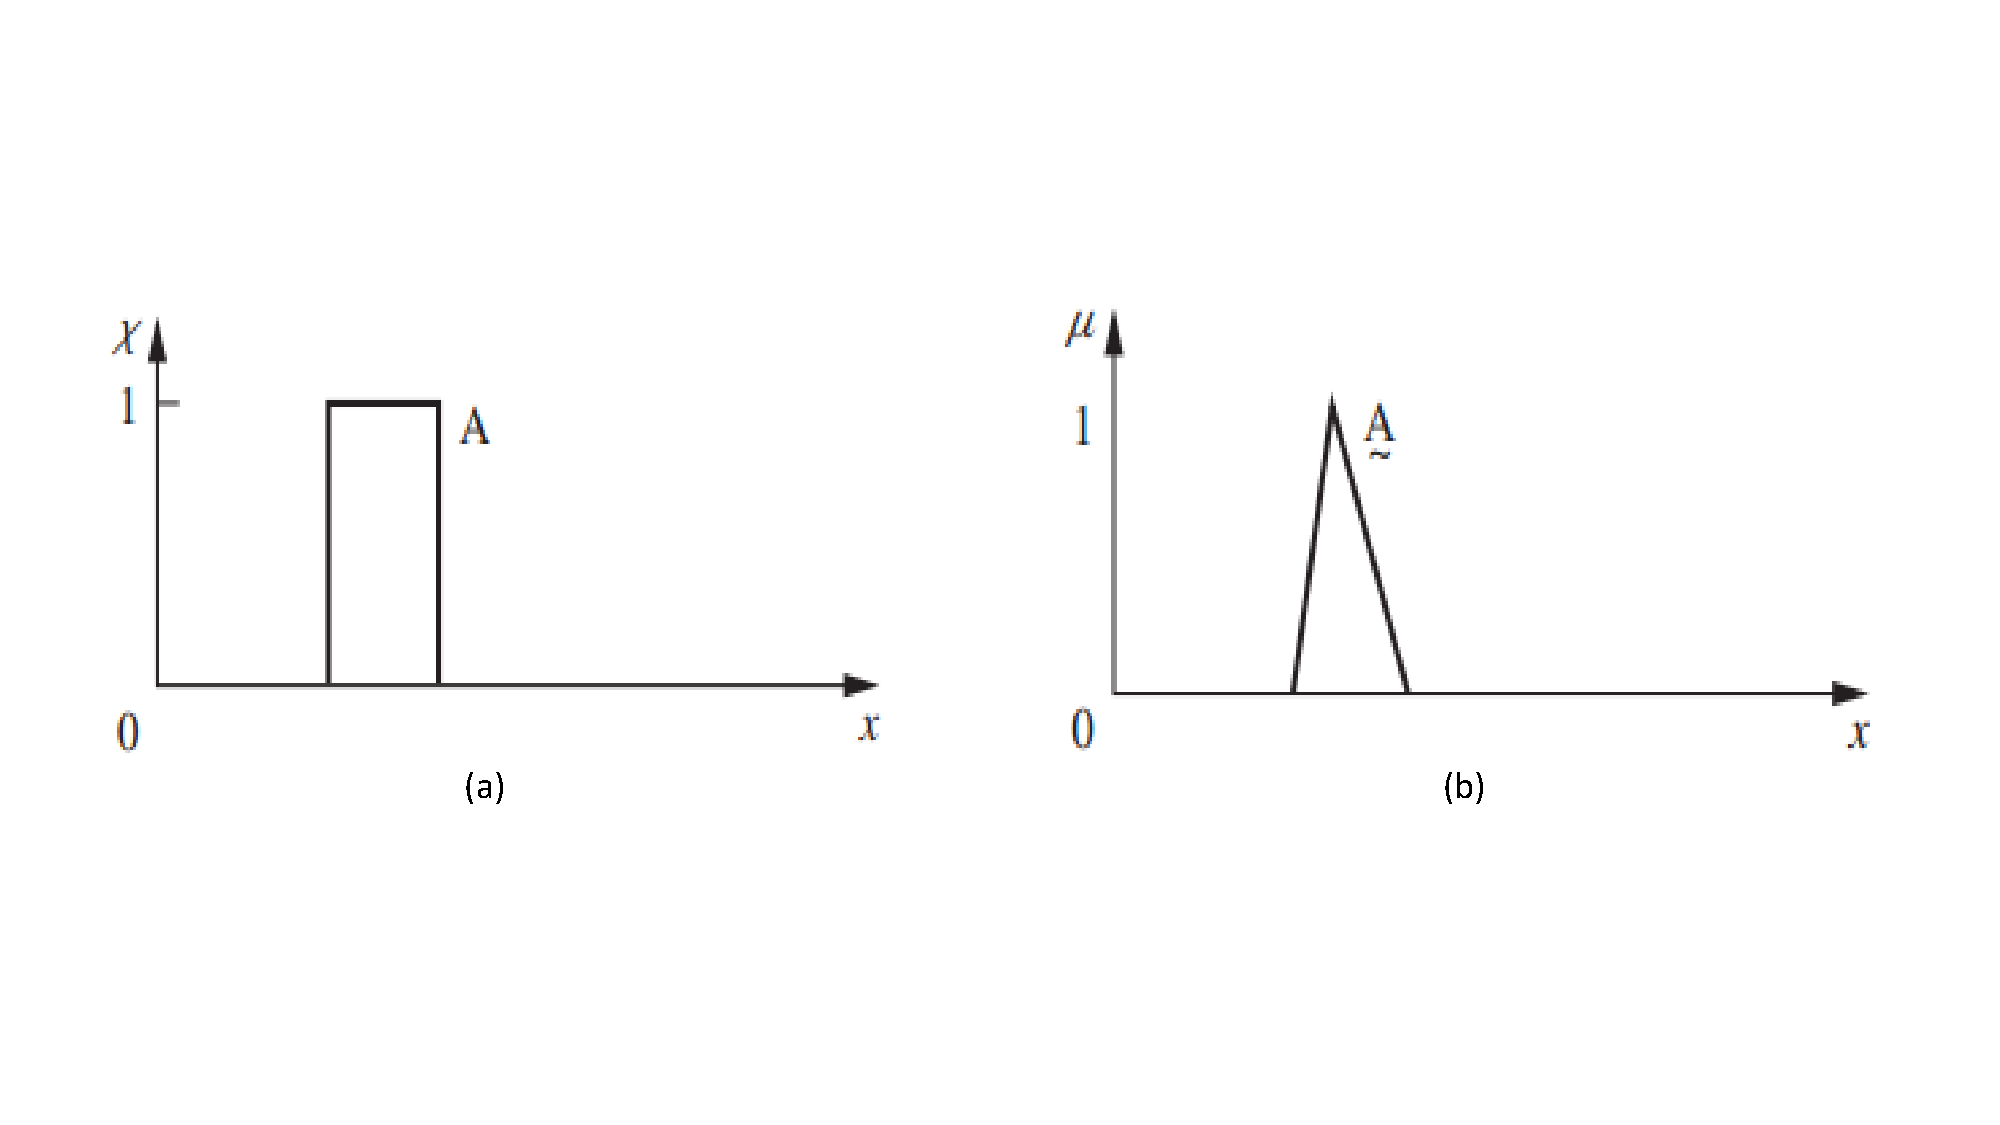
\includegraphics[width=1\linewidth]{images/fungsi_keanggotaan_fuzzy.pdf}
    \caption{Perbedaan fungsi keanggotaan antara (a) Himpunan Tegas dan (b) Himpunan Kabur \cite{ross_fuzzy_2016}}
    \label{fig:keanggotaan_fuzzy}
\end{figure}

\subsubsection{Variabel Linguistik (\textit{Linguistic Variable})}
Variabel linguistik adalah variabel yang nilainya dinyatakan dalam bentuk istilah bahasa alami seperti “rendah”, “sedang”, “tinggi”, atau “panas”. Setiap istilah linguistik direpresentasikan oleh satu himpunan fuzzy dengan fungsi keanggotaan tertentu \cite{zadeh_concept_1975}.
Sebagai contoh, untuk variabel “suhu”, dapat didefinisikan tiga istilah linguistik: “dingin”, “hangat”, dan “panas”, yang masing-masing memiliki fungsi keanggotaan berbeda terhadap domain suhu.

\subsubsection{Label Linguistik (\textit{Linguistic Label})}
Label linguistik atau nilai linguistik atau disebut juga sebagai terma merupakan istilah spesifik yang digunakan untuk menyatakan nilai dari suatu variabel linguistik \cite{noauthor_linguistic_nodate,rinaldi_munir_logika_2021}. Misalnya, dalam variabel linguistik “kecepatan mobil”, label linguistik yang digunakan dapat berupa “lambat”, “sedang”, dan “cepat”. Label ini digunakan dalam perumusan aturan fuzzy seperti “IF kecepatan tinggi THEN jarak pengereman jauh”.

\subsubsection{Operator Logika Fuzzy}
Operator logika fuzzy digunakan untuk mengombinasikan atau memodifikasi nilai keanggotaan. Operator dasar yang digunakan meliputi:
\begin{itemize}
    \item \textbf{AND (Konjungsi)} – biasanya direpresentasikan dengan operator minimum.
    \item \textbf{OR (Disjungsi)} – direpresentasikan dengan operator maksimum.
    \item \textbf{NOT (Negasi)} – direpresentasikan dengan operator komplemen, yaitu \(1 - \mu_A(x)\).
\end{itemize}
Operator-operator ini merupakan dasar dalam pembentukan aturan fuzzy dan proses inferensi.

\subsubsection{Inferensi Fuzzy (\textit{Fuzzy Inference})}
Inferensi fuzzy adalah proses penalaran yang digunakan untuk menghasilkan kesimpulan berdasarkan serangkaian aturan fuzzy. Proses ini menggunakan nilai-nilai keanggotaan dari input dan aturan linguistik untuk menentukan output sistem.
Metode inferensi yang umum digunakan antara lain metode Mamdani dan metode Sugeno.

\subsubsection{Defuzzifikasi (\textit{Defuzzification})}
Defuzzifikasi adalah tahap akhir dalam sistem inferensi fuzzy yang berfungsi untuk mengubah hasil fuzzy (bernilai kontinu antara 0 dan 1) menjadi nilai tegas (crisp output). Nilai ini digunakan untuk pengambilan keputusan atau pengendalian aktual. Beberapa metode populer adalah \textit{centroid}, \textit{bisector}, dan \textit{mean of maximum}.

\subsection{Derajat dan Fungsi Keanggotaan}

Dalam logika klasik, hubungan antara suatu elemen dengan himpunan bersifat biner: suatu elemen hanya dapat menjadi anggota atau bukan anggota dari himpunan tersebut. Secara matematis, hal ini dinyatakan dengan fungsi keanggotaan \(\mu_A(x)\) yang hanya mengambil dua nilai:
\[
    \mu_A(x) =
    \begin{cases}
        1, & \text{jika } x \in A,    \\
        0, & \text{jika } x \notin A.
    \end{cases}
\]
Pendekatan seperti ini sesuai untuk sistem dengan batasan tegas, tetapi menjadi tidak memadai ketika konsep yang dimodelkan bersifat relatif atau samar. Misalnya, tidak ada batas universal yang pasti untuk menentukan kapan suatu suhu dapat disebut “panas” atau “dingin”.

Logika fuzzy memperluas konsep tersebut dengan memperkenalkan \textbf{derajat keanggotaan} (\textit{degree of membership}), yaitu ukuran sejauh mana suatu elemen termasuk dalam sebuah himpunan fuzzy. Nilai keanggotaan dinyatakan dalam interval kontinu \([0,1]\), di mana:
\[
    \mu_A: X \rightarrow [0,1].
\]
Nilai \(\mu_A(x)=0\) menunjukkan bahwa elemen \(x\) tidak termasuk dalam himpunan fuzzy \(A\), \(\mu_A(x)=1\) menunjukkan keanggotaan penuh, sedangkan \(0 < \mu_A(x) < 1\) menyatakan tingkat keanggotaan parsial. Dengan demikian, derajat keanggotaan merepresentasikan intensitas atau kekuatan hubungan antara elemen dan konsep linguistik yang diwakili oleh himpunan fuzzy \cite{ross_fuzzy_2016}.

Sebagai contoh, pada konsep linguistik “suhu panas”, setiap nilai suhu \(x\) memiliki derajat keanggotaan yang menyatakan seberapa “panas” suhu tersebut:
\[
    \mu_{\text{panas}}(25) = 0.3, \quad
    \mu_{\text{panas}}(28) = 0.7, \quad
    \mu_{\text{panas}}(35) = 1.0.
\]
Artinya, suhu 25°C hanya sedikit panas, 28°C cukup panas, dan 35°C sepenuhnya panas. Nilai-nilai ini ditentukan oleh \textbf{fungsi keanggotaan} yang mendeskripsikan hubungan kuantitatif antara variabel numerik dan persepsi linguistik.

\textbf{Fungsi keanggotaan} (\textit{membership function}) merupakan komponen inti dalam logika fuzzy yang memetakan setiap elemen dari semesta pembicaraan (\textit{universe of discourse}) ke nilai derajat keanggotaan pada interval \([0,1]\). Bentuk fungsi keanggotaan menentukan karakteristik transisi antara “tidak termasuk” dan “sepenuhnya termasuk” dalam suatu himpunan fuzzy, sehingga berperan penting dalam representasi semantik dan hasil inferensi fuzzy.

\subsubsection{Bentuk Umum Fungsi Keanggotaan}

Beberapa bentuk fungsi keanggotaan yang umum digunakan antara lain \cite{saputra_optimasi_2019}.

\begin{itemize}
    \item \textbf{Fungsi Linear Naik (Increasing Linear Membership Function)}
          Fungsi ini digunakan untuk merepresentasikan kenaikan derajat keanggotaan secara linier dari 0 ke 1 pada interval \((a,b)\).
          Dirumuskan sebagai:
          \[
              \mu_A(x) =
              \begin{cases}
                  0,               & x \leq a,  \\
                  \frac{x-a}{b-a}, & a < x < b, \\
                  1,               & x \geq b.
              \end{cases}
          \]
          Fungsi ini cocok untuk memodelkan konsep linguistik seperti “semakin besar”, “semakin cepat”, atau “semakin tinggi”.

    \item \textbf{Fungsi Linear Turun (Decreasing Linear Membership Function)}
          Fungsi ini merupakan kebalikan dari fungsi linear naik, digunakan untuk menunjukkan penurunan derajat keanggotaan secara linier dari 1 ke 0 pada interval \((a,b)\).
          Didefinisikan sebagai:
          \[
              \mu_A(x) =
              \begin{cases}
                  1,               & x \leq a,  \\
                  \frac{b-x}{b-a}, & a < x < b, \\
                  0,               & x \geq b.
              \end{cases}
          \]
          Umumnya digunakan untuk merepresentasikan istilah seperti “semakin kecil”, “semakin lambat”, atau “semakin rendah”.

    \item \textbf{Fungsi Segitiga (Triangular Membership Function)}
          Didefinisikan oleh tiga parameter \((a,b,c)\) dengan bentuk segitiga, di mana \(a\) dan \(c\) adalah batas bawah dan atas, dan \(b\) titik puncak:
          \[
              \mu_A(x) =
              \begin{cases}
                  0,               & x \leq a \text{ atau } x \geq c, \\
                  \frac{x-a}{b-a}, & a < x \leq b,                    \\
                  \frac{c-x}{c-b}, & b < x < c.
              \end{cases}
          \]
          Fungsi ini sederhana dan efisien secara komputasi, cocok untuk sistem real-time.

    \item \textbf{Fungsi Trapesium (Trapezoidal Membership Function)}
          Merupakan generalisasi fungsi segitiga dengan empat parameter \((a,b,c,d)\):
          \[
              \mu_A(x) =
              \begin{cases}
                  0,               & x \leq a \text{ atau } x \geq d, \\
                  \frac{x-a}{b-a}, & a < x \leq b,                    \\
                  1,               & b < x \leq c,                    \\
                  \frac{d-x}{d-c}, & c < x < d.
              \end{cases}
          \]
          Umum digunakan ketika terdapat rentang nilai yang dianggap sepenuhnya memenuhi suatu kategori linguistik.

    \item \textbf{Fungsi Gaussian (Gaussian Membership Function)}
          Memberikan transisi halus dan kontinu dengan dua parameter, mean (\(c\)) dan standar deviasi (\(\sigma\)):
          \[
              \mu_A(x) = e^{-\frac{1}{2}\left(\frac{x - c}{\sigma}\right)^2}.
          \]
          Cocok untuk data berdistribusi normal dan sistem dengan kebutuhan inferensi yang lembut.

    \item \textbf{Fungsi Sigmoid (Sigmoidal Membership Function)}
          Digunakan untuk memodelkan kenaikan atau penurunan bertahap tanpa batas tegas:
          \[
              \mu_A(x) = \frac{1}{1 + e^{-a(x-c)}},
          \]
          dengan \(a\) mengatur kemiringan kurva dan \(c\) titik tengah transisi.
\end{itemize}

Gambar
\begin{figure}[H]
    \centering
    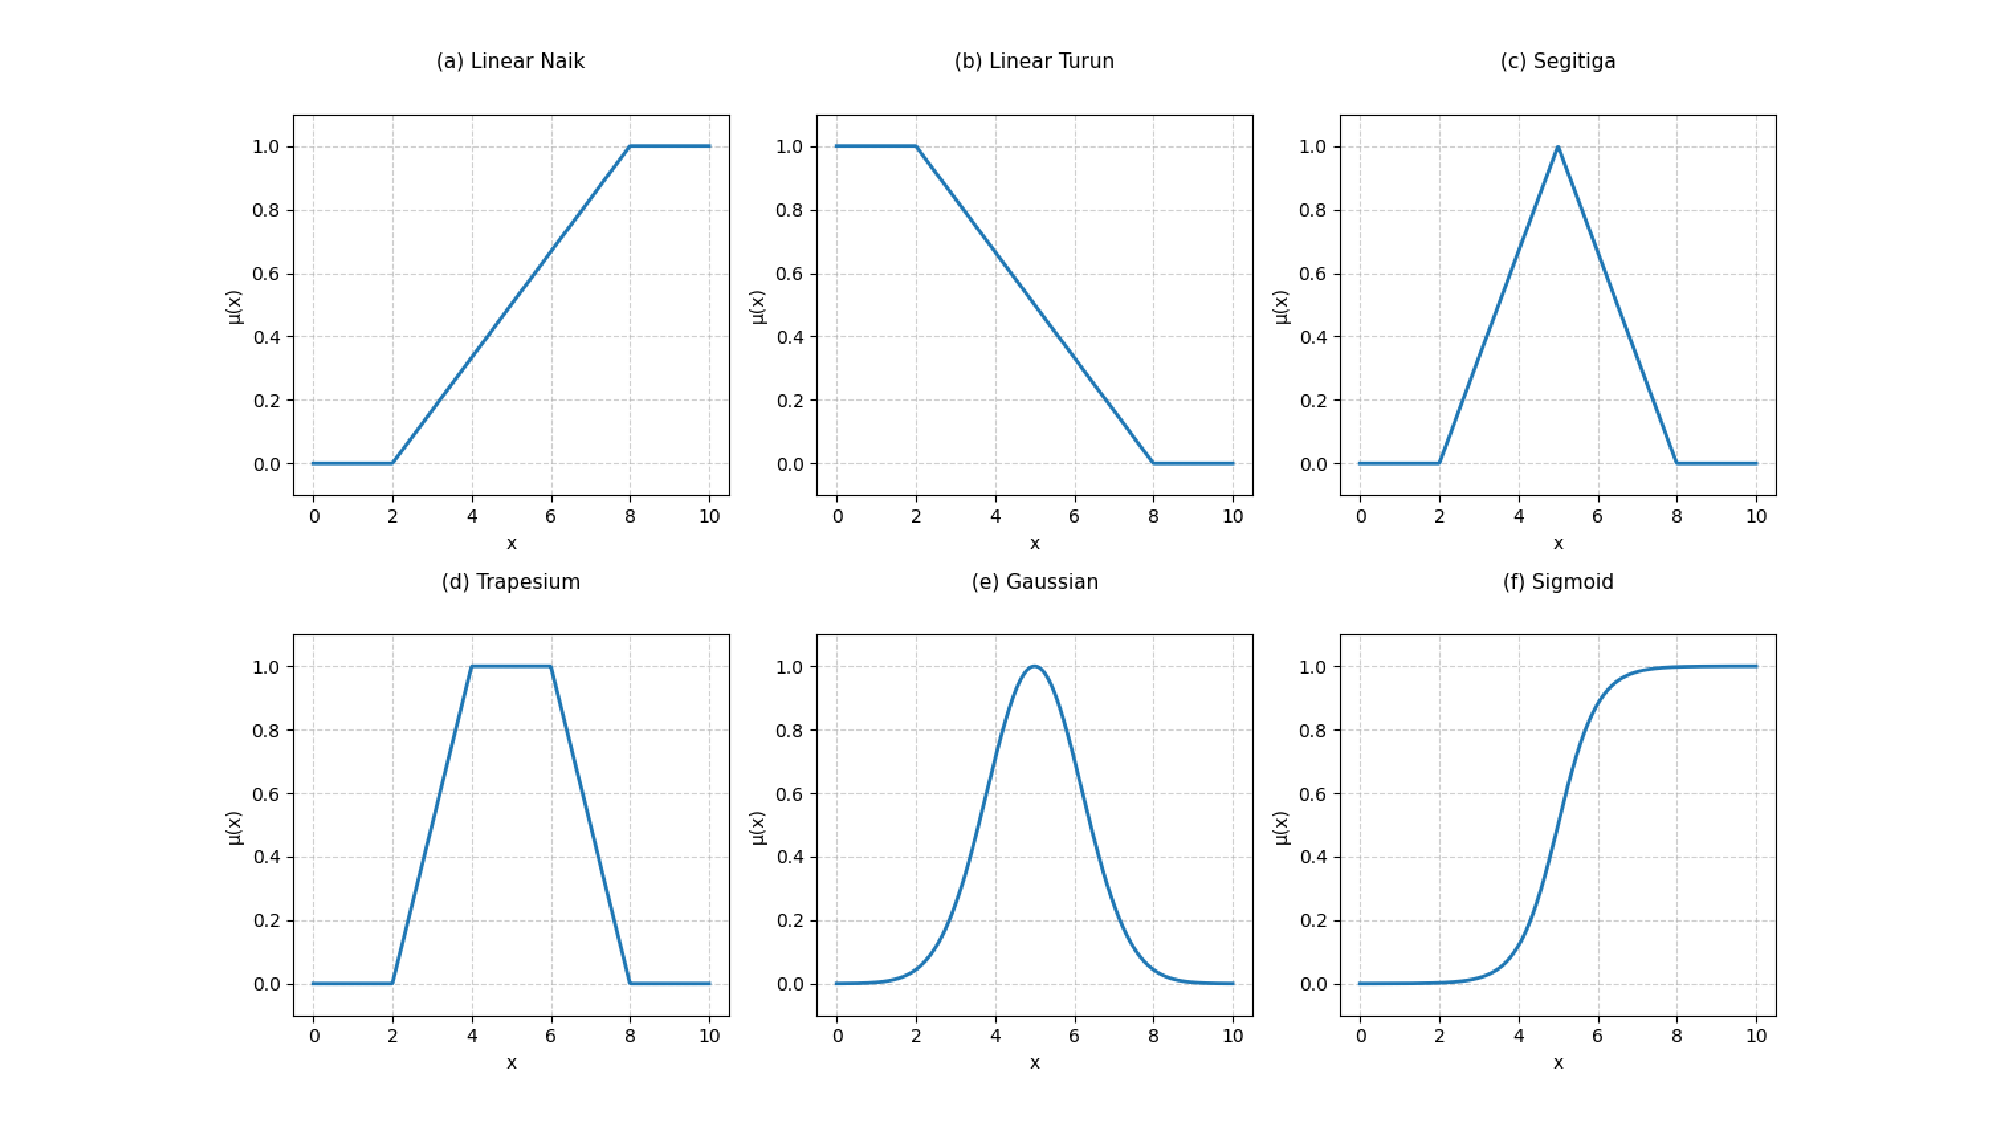
\includegraphics[width=1\linewidth]{images/semua_fungsi_keanggotaan.pdf}
    \caption{Berbagai bentuk fungsi keanggotaan (\textit{membership function}) dalam logika fuzzy:
        (a) linear naik,
        (b) linear turun,
        (c) segitiga,
        (d) trapesium,
        (e) Gaussian, dan
        (f) sigmoid.
        Setiap bentuk menunjukkan cara berbeda dalam memetakan nilai crisp ke derajat keanggotaan dalam interval kontinu [0,1].}

    \label{fig:semua_keanggotaan}
\end{figure}


\subsubsection{Pertimbangan dalam Pemilihan Fungsi Keanggotaan}

Pemilihan bentuk fungsi keanggotaan bergantung pada:
\begin{enumerate}
    \item \textbf{Karakteristik data}, menentukan apakah diperlukan transisi halus (Gaussian) atau linier (segitiga/trapesium);
    \item \textbf{Kebutuhan komputasi}, fungsi sederhana lebih efisien untuk sistem waktu nyata;
    \item \textbf{Interpretasi linguistik}, fungsi harus merepresentasikan makna istilah secara intuitif;
    \item \textbf{Tujuan aplikasi}, misalnya kontrol presisi tinggi memerlukan bentuk fungsi yang lebih kompleks.
\end{enumerate}

Dengan demikian, derajat keanggotaan dan fungsi keanggotaan merupakan dua aspek tak terpisahkan dalam teori himpunan fuzzy. Derajat keanggotaan memformalkan intensitas keanggotaan suatu elemen, sementara fungsi keanggotaan menentukan bagaimana intensitas tersebut dibentuk secara matematis dan ditafsirkan secara semantik.

\subsection{Variabel Linguistik dan Himpunan Fuzzy}
Variabel linguistik (\textit{linguistic variable}) adalah konsep fundamental dalam sistem logika fuzzy yang diperkenalkan oleh Lotfi A. Zadeh \cite{zadeh_concept_1975}. Berbeda dengan variabel numerik yang bernilai eksak, variabel linguistik memiliki nilai berupa kata-kata atau istilah dalam bahasa alami, seperti “rendah”, “sedang”, atau “tinggi”. Setiap istilah linguistik tersebut diwakili oleh suatu \textbf{himpunan fuzzy} yang memiliki fungsi keanggotaan tertentu terhadap domain numeriknya.

Secara formal, variabel linguistik \(V\) dapat dinyatakan sebagai suatu tuple:
\[
    V = (x, T(x), U, G, M),
\]
dengan:
\begin{itemize}
    \item \(x\) : nama variabel linguistik, misalnya “suhu” atau “kecepatan”;
    \item \(T(x)\) : himpunan istilah linguistik yang dapat digunakan untuk menggambarkan nilai dari \(x\), misalnya \(T(\text{suhu}) = \{\text{dingin, hangat, panas}\}\);
    \item \(U\) : semesta pembicaraan (\textit{universe of discourse}), yaitu domain numerik dari variabel tersebut, misalnya \(U = [0, 50]\) untuk suhu dalam °C;
    \item \(G\) : aturan sintaktik yang menentukan bagaimana istilah linguistik kompleks dapat dibentuk (misalnya “sangat panas” atau “tidak dingin”);
    \item \(M\) : aturan semantik yang memetakan istilah linguistik ke himpunan fuzzy di \(U\) melalui fungsi keanggotaan.
\end{itemize}

Dengan demikian, setiap nilai linguistik \(L \in T(x)\) direpresentasikan oleh sebuah himpunan fuzzy \(A_L\) pada domain \(U\), dengan fungsi keanggotaan \(\mu_{A_L}(u)\). Nilai \(\mu_{A_L}(u)\) menunjukkan seberapa besar derajat kebenaran bahwa nilai \(u\) dapat dikatakan sebagai \(L\).

Sebagai contoh, untuk variabel linguistik “suhu”, dengan semesta pembicaraan \(U = [0, 50]\), dapat didefinisikan tiga himpunan fuzzy:
\[
    T(\text{suhu}) = \{\text{dingin}, \text{hangat}, \text{panas}\}.
\]
Masing-masing himpunan fuzzy memiliki fungsi keanggotaan seperti berikut:
\[
    \mu_{\text{dingin}}(x), \quad \mu_{\text{hangat}}(x), \quad \mu_{\text{panas}}(x).
\]
Nilai-nilai ini mungkin didefinisikan sebagai fungsi segitiga atau trapesium pada domain suhu, misalnya:
\[
    \mu_{\text{panas}}(x) =
    \begin{cases}
        0,                 & x \leq 25,      \\
        \frac{x - 25}{10}, & 25 < x \leq 35, \\
        1,                 & x > 35.
    \end{cases}
\]

Dengan pendekatan seperti ini, nilai suhu \(x = 30^\circ C\) dapat memiliki derajat keanggotaan \(\mu_{\text{hangat}}(30) = 0.6\) dan \(\mu_{\text{panas}}(30) = 0.3\). Artinya, suhu 30°C dapat dianggap “agak hangat” sekaligus “mulai panas”, tergantung konteks interpretasinya. Ini menggambarkan kekuatan representasi fuzzy: ia memungkinkan makna linguistik direpresentasikan secara numerik tanpa kehilangan ambiguitas alami bahasa manusia.

\subsubsection{Peran Variabel Linguistik dalam Sistem Fuzzy}
Dalam sistem inferensi fuzzy, variabel linguistik digunakan untuk membentuk aturan logika berbasis bahasa alami, misalnya:
\[
    \text{IF suhu is panas THEN kipas is cepat}.
\]
Pada contoh ini, “suhu” dan “kipas” adalah variabel linguistik, sedangkan “panas” dan “cepat” adalah istilah linguistik yang memiliki representasi fuzzy masing-masing. Mesin inferensi fuzzy kemudian melakukan perhitungan menggunakan derajat keanggotaan dari istilah-istilah tersebut untuk menghasilkan kesimpulan yang bersifat numerik.

Pendekatan ini memungkinkan sistem fuzzy menjembatani antara logika formal dan bahasa alami. Sistem dapat memahami dan mengoperasikan pernyataan yang bersifat samar seperti “cukup cepat” atau “agak panas”, sesuatu yang tidak mungkin dilakukan oleh logika biner klasik.

\subsubsection{Hierarki dan Kombinasi Nilai Linguistik}
Nilai linguistik tidak selalu bersifat atomik. Dalam banyak kasus, istilah seperti “sangat tinggi”, “agak rendah”, atau “tidak panas” dibentuk melalui modifikasi terhadap himpunan fuzzy dasar menggunakan \textit{linguistic hedges} (kata pengubah).
Contoh fungsi pengubah yang umum digunakan:
\begin{itemize}
    \item “\textit{Sangat}” (\textit{very}) dapat dimodelkan dengan operasi kuadrat: \(\mu_{\text{sangat }A}(x) = [\mu_A(x)]^2\).
    \item “\textit{Agak}” (\textit{somewhat}) dimodelkan dengan akar kuadrat: \(\mu_{\text{agak }A}(x) = [\mu_A(x)]^{1/2}\).
    \item “\textit{Tidak}” (\textit{not}) direpresentasikan dengan komplemen fuzzy: \(\mu_{\text{tidak }A}(x) = 1 - \mu_A(x)\).
\end{itemize}

Dengan demikian, istilah linguistik kompleks dapat dibangun secara sistematis dari himpunan fuzzy dasar tanpa kehilangan interpretasi semantik aslinya.

\subsection{Operasi Logika Fuzzy}

Operasi dasar dalam logika fuzzy merupakan generalisasi dari operasi logika biner pada sistem klasik. Dalam logika klasik, nilai kebenaran suatu proposisi hanya dapat bernilai 0 (salah) atau 1 (benar), dan operasi logikanya didefinisikan secara tegas. Namun dalam logika fuzzy, setiap proposisi memiliki derajat kebenaran kontinu pada interval \([0,1]\), sehingga operasi logika perlu didefinisikan ulang agar dapat menangani nilai antara.

Jika \(\mu_A(x)\) dan \(\mu_B(x)\) masing-masing menyatakan derajat keanggotaan elemen \(x\) terhadap himpunan fuzzy \(A\) dan \(B\), maka hasil operasi logika fuzzy dinyatakan dengan fungsi baru \(\mu_{A * B}(x)\), di mana simbol \(*\) bergantung pada jenis operasi yang digunakan.

\subsubsection{Konjungsi Fuzzy (Operasi AND)}
Konjungsi dalam logika fuzzy mewakili operasi \textbf{irisan} (\textit{intersection}) antara dua himpunan fuzzy. Secara umum, konjungsi diimplementasikan dengan menggunakan \textit{t-norm} (triangular norm), yaitu fungsi biner \(T: [0,1]^2 \to [0,1]\) yang memenuhi empat sifat utama:
\begin{enumerate}
    \item \textbf{Komutatif:} \(T(a,b) = T(b,a)\)
    \item \textbf{Asosiatif:} \(T(a, T(b,c)) = T(T(a,b), c)\)
    \item \textbf{Monotonik:} Jika \(a_1 \leq a_2\) dan \(b_1 \leq b_2\), maka \(T(a_1,b_1) \leq T(a_2,b_2)\)
    \item \textbf{Batas identitas:} \(T(a,1) = a\)
\end{enumerate}

Bentuk \textit{t-norm} yang umum digunakan antara lain:
\begin{itemize}
    \item \textbf{Minimum:} \(T_{\min}(a,b) = \min(a,b)\)
    \item \textbf{Produk aljabar:} \(T_{\text{prod}}(a,b) = a \times b\)
    \item \textbf{Bounded difference:} \(T_{\text{bd}}(a,b) = \max(0, a+b-1)\)
\end{itemize}

Operator minimum paling banyak digunakan karena sederhana dan mudah diinterpretasikan: hasil konjungsi fuzzy adalah nilai keanggotaan terendah dari kedua himpunan pada titik tersebut.
Sebagai contoh:
\begin{equation}
    \label{eq:konjungsi_minimum}
    \mu_{A \cap B}(x) = \min(\mu_A(x), \mu_B(x)).
\end{equation}

Sebaliknya, operator produk memberikan hasil yang lebih halus secara matematis, cocok untuk sistem yang membutuhkan transisi mulus dan komputasi probabilistik:
\[
    \mu_{A \cap B}(x) = \mu_A(x) \times \mu_B(x).
\]

\subsubsection{Disjungsi Fuzzy (Operasi OR)}
Disjungsi merepresentasikan operasi \textbf{gabungan} (\textit{union}) antara dua himpunan fuzzy. Dalam konteks fuzzy, disjungsi didefinisikan melalui \textit{t-conorm} (atau \textit{s-norm}), yaitu fungsi \(S: [0,1]^2 \to [0,1]\) yang memenuhi:
\begin{enumerate}
    \item \textbf{Komutatif:} \(S(a,b) = S(b,a)\)
    \item \textbf{Asosiatif:} \(S(a, S(b,c)) = S(S(a,b), c)\)
    \item \textbf{Monotonik:} Jika \(a_1 \leq a_2\) dan \(b_1 \leq b_2\), maka \(S(a_1,b_1) \leq S(a_2,b_2)\)
    \item \textbf{Batas identitas:} \(S(a,0) = a\)
\end{enumerate}

Beberapa bentuk \textit{t-conorm} yang umum digunakan:
\begin{itemize}
    \item \textbf{Maksimum:} \(S_{\max}(a,b) = \max(a,b)\)
    \item \textbf{Penjumlahan aljabar:} \(S_{\text{sum}}(a,b) = a + b - (a \times b)\)
    \item \textbf{Bounded sum:} \(S_{\text{bs}}(a,b) = \min(1, a + b)\)
\end{itemize}

Operator maksimum paling umum digunakan karena interpretasinya intuitif — hasil disjungsi fuzzy adalah nilai keanggotaan tertinggi antara dua himpunan pada titik yang sama:
\[
    \mu_{A \cup B}(x) = \max(\mu_A(x), \mu_B(x)).
\]
Sementara penjumlahan aljabar lebih cocok untuk sistem yang menghendaki peningkatan derajat keanggotaan tanpa mencapai saturasi terlalu cepat.

\subsubsection{Negasi Fuzzy (Operasi NOT)}
Negasi fuzzy (\textit{fuzzy complement}) adalah operasi unary yang merepresentasikan kebalikan atau penyangkalan terhadap suatu himpunan fuzzy.
Negasi fuzzy paling sederhana, dan paling sering digunakan, adalah:
\[
    \mu_{\neg A}(x) = 1 - \mu_A(x).
\]
Namun, terdapat bentuk negasi yang lebih umum, disebut \textit{strong negation}, dengan sifat:
\begin{enumerate}
    \item \(\text{N}(0) = 1\) dan \(\text{N}(1) = 0\),
    \item \(\text{N}\) bersifat monoton menurun,
    \item \(\text{N}(\text{N}(a)) = a\).
\end{enumerate}
Contoh lain:
\[
    \text{N}(a) = (1 - a)^k, \quad k > 0.
\]
Nilai \(k\) menentukan seberapa cepat negasi meningkat; semakin besar \(k\), semakin tajam perubahan dari 1 ke 0.

\subsubsection{Operasi Gabungan dan Himpunan Turunan}
Selain tiga operasi dasar di atas, logika fuzzy juga mengenal operasi turunan seperti:
\begin{itemize}
    \item \textbf{Difference (selisih fuzzy):}
          \[
              \mu_{A - B}(x) = \min(\mu_A(x), 1 - \mu_B(x))
          \]
    \item \textbf{Complemented union (gabungan dengan negasi):}
          \[
              \mu_{A \cup \neg B}(x) = \max(\mu_A(x), 1 - \mu_B(x))
          \]
\end{itemize}
Operasi-operasi ini sering digunakan pada tahap inferensi fuzzy untuk mengombinasikan aturan-aturan yang bersifat saling meniadakan atau memperkuat.

\subsubsection{Pertimbangan Pemilihan Operator}
Pemilihan operator fuzzy (t-norm, t-conorm, dan negasi) mempengaruhi hasil inferensi dan sensitivitas sistem secara keseluruhan. Secara umum:
\begin{itemize}
    \item Operator \textbf{minimum–maksimum} cocok untuk sistem berbasis aturan linguistik sederhana karena interpretasinya intuitif.
    \item Operator \textbf{produk–penjumlahan} lebih cocok untuk sistem yang membutuhkan transisi halus dan perhitungan berbasis probabilistik.
    \item Operator \textbf{bounded} digunakan ketika nilai keanggotaan perlu dibatasi agar tidak keluar dari interval [0,1] akibat akumulasi nilai ekstrem.
\end{itemize}

\subsection{Aturan Fuzzy dan Sistem Inferensi Fuzzy}

Sistem inferensi fuzzy (\textit{Fuzzy Inference System}, FIS) merupakan mekanisme utama dalam penerapan logika fuzzy yang berfungsi untuk menalar atau mengambil keputusan berdasarkan aturan berbasis bahasa alami. Prinsip dasarnya adalah mengubah input numerik menjadi representasi linguistik, memprosesnya melalui seperangkat aturan \textit{IF–THEN}, kemudian menghasilkan keluaran yang juga bersifat linguistik atau numerik.

\subsubsection{Struktur Aturan Fuzzy}

Aturan fuzzy secara umum dituliskan dalam bentuk:
\[
    \text{IF } x_1 \text{ is } A_1^k \text{ AND } x_2 \text{ is } A_2^k \text{ AND } \dots \text{ THEN } y \text{ is } B^k,
\]
dengan:
\begin{itemize}
    \item \(x_i\) adalah variabel input,
    \item \(A_i^k\) adalah himpunan fuzzy yang merepresentasikan istilah linguistik dari \(x_i\),
    \item \(B^k\) adalah himpunan fuzzy atau fungsi yang merepresentasikan keluaran,
    \item indeks \(k\) menunjukkan aturan ke-\(k\) dari keseluruhan basis aturan fuzzy.
\end{itemize}

Contohnya, untuk sistem pengendali suhu kipas:
\[
    \text{IF suhu tinggi AND kelembapan rendah THEN kecepatan kipas cepat.}
\]
Bagian “\textit{IF suhu tinggi AND kelembapan rendah}” disebut \textbf{premis} (antecedent), sedangkan “\textit{THEN kecepatan kipas cepat}” disebut \textbf{konsekuen} (consequent).

\subsubsection{Tahapan Proses Inferensi Fuzzy}

Sistem inferensi fuzzy secara umum melibatkan empat tahap utama:

\begin{enumerate}
    \item \textbf{Fuzzifikasi (Fuzzification)}
          Pada tahap ini, nilai input numerik diubah menjadi derajat keanggotaan terhadap himpunan fuzzy yang sesuai.
          Misalnya, suhu \(x = 30^\circ C\) dapat memiliki \(\mu_{\text{hangat}}(x) = 0.6\) dan \(\mu_{\text{panas}}(x) = 0.3\).

    \item \textbf{Evaluasi Aturan (Rule Evaluation)}
          Setiap aturan dievaluasi dengan menggunakan operator fuzzy (biasanya t-norm untuk AND dan t-conorm untuk OR).
          Misalnya, untuk aturan:
          \[
              \text{IF suhu is panas AND kelembapan is rendah THEN kipas is cepat,}
          \]
          derajat kebenaran dari premis dihitung sebagai:
          \[
              \alpha_k = \min(\mu_{\text{panas}}(x_1), \mu_{\text{rendah}}(x_2)).
          \]
          Nilai \(\alpha_k\) disebut \textit{firing strength} atau tingkat aktivasi aturan ke-\(k\).

    \item \textbf{Agregasi (Rule Aggregation)}
          Hasil dari setiap aturan dikombinasikan untuk membentuk keluaran fuzzy tunggal. Jika setiap aturan menghasilkan himpunan fuzzy \(B^k\) dengan tingkat aktivasi \(\alpha_k\), maka hasil agregasinya diberikan oleh:
          \[
              \mu_{B_{\text{agregat}}}(y) = \max_k [ \min(\alpha_k, \mu_{B^k}(y)) ].
          \]
          Proses ini mencerminkan bahwa keluaran akhir dipengaruhi oleh semua aturan yang “menyala” (aktif).

    \item \textbf{Defuzzifikasi (Defuzzification)}
          Jika keluaran sistem berupa himpunan fuzzy, maka perlu dikonversi menjadi nilai numerik tegas (crisp value) agar dapat digunakan dalam sistem nyata.
          Beberapa metode umum antara lain: metode centroid, bisektor, dan mean of maxima.
\end{enumerate}

\subsubsection{Metode Inferensi Fuzzy}

Terdapat beberapa pendekatan dalam sistem inferensi fuzzy, namun dua metode yang paling umum adalah \textbf{Mamdani} dan \textbf{Sugeno}.

\paragraph{1. Metode Mamdani}
Metode Mamdani (1975) adalah pendekatan klasik yang menggunakan himpunan fuzzy baik pada premis maupun konsekuen. Keluaran dari setiap aturan berupa himpunan fuzzy yang kemudian diagregasi dan didefuzzifikasi.
Aturan Mamdani berbentuk:
\[
    \text{IF } x_1 \text{ is } A_1^k \text{ AND } x_2 \text{ is } A_2^k \text{ THEN } y \text{ is } B^k.
\]
Derajat aktivasi aturan ke-\(k\):
\[
    \alpha_k = T(\mu_{A_1^k}(x_1), \mu_{A_2^k}(x_2), \dots),
\]
dengan \(T\) merupakan operator t-norm (biasanya minimum atau produk).
Keluaran fuzzy dari setiap aturan kemudian dimodifikasi menggunakan metode \textit{implication} seperti:
\[
    \mu_{B'^k}(y) = \min(\alpha_k, \mu_{B^k}(y)),
\]
dan hasil akhir sistem diperoleh melalui agregasi semua \(\mu_{B'^k}(y)\).
Metode Mamdani banyak digunakan untuk sistem kontrol karena interpretasinya intuitif dan mudah dihubungkan dengan pengetahuan pakar manusia.

\paragraph{2. Metode Sugeno (Takagi–Sugeno–Kang)}
Metode Sugeno (1985) menggunakan konsekuen yang berupa fungsi matematis, bukan himpunan fuzzy. Aturan umum ditulis sebagai:
\[
    \text{IF } x_1 \text{ is } A_1^k \text{ AND } x_2 \text{ is } A_2^k \text{ THEN } y = f_k(x_1, x_2),
\]
di mana \(f_k(x_1, x_2)\) biasanya berbentuk fungsi linear:
\[
    f_k(x_1, x_2) = p_k x_1 + q_k x_2 + r_k,
\]
dengan \(p_k, q_k, r_k\) sebagai parameter.
Derajat aktivasi \(\alpha_k\) dihitung sama seperti pada Mamdani, tetapi keluaran sistem diperoleh melalui rata-rata berbobot:
\begin{equation}
    y^* = \frac{\sum_{k=1}^n \alpha_k f_k(x_1, x_2)}{\sum_{k=1}^n \alpha_k}.
    \label{eq:defuzzifikasi_sugeno}
\end{equation}


Metode Sugeno lebih efisien secara komputasi dan cocok untuk sistem adaptif, terutama ketika digabungkan dengan teknik pembelajaran seperti ANFIS (Adaptive Neuro-Fuzzy Inference System).

\subsubsection{Perbandingan Mamdani dan Sugeno}
Tabel \ref{tab:perbedaan_masu} membandingkan antara metode Mamdani dan Sugeno.
\begin{table}[H]
    \centering
    \caption{Perbedaan antara Mamdani dan Sugeno}
    \label{tab:perbedaan_masu}

    \begin{tabular}{|p{3cm}|p{5cm}|p{5cm}|}
        \hline
        \textbf{Aspek}                                    & \textbf{Mamdani}                    & \textbf{Sugeno}                           \\ \hline
        \textbf{Bentuk Konsekuen}                         & Himpunan fuzzy                      & Fungsi linear atau konstanta              \\ \hline
        \textbf{Defuzzifikasi}                            & Diperlukan (mis. centroid)          & Tidak diperlukan (hasil langsung numerik) \\ \hline
        \textbf{Kesesuaian untuk Interpretasi Linguistik} & Sangat tinggi, mudah dipahami pakar & Lebih matematis, kurang intuitif          \\ \hline
        \textbf{Efisiensi Komputasi}                      & Relatif lebih berat                 & Lebih cepat, cocok untuk sistem real-time \\ \hline
        \textbf{Aplikasi Umum}                            & Kontrol industri, sistem pakar      & Sistem adaptif, prediksi, dan optimasi    \\ \hline
    \end{tabular}

\end{table}


\subsection{Keunggulan dan Keterbatasan Logika Fuzzy}
Logika fuzzy unggul dalam menangani data yang tidak pasti, ambigu, atau bersifat linguistik. Ia mampu memodelkan cara berpikir manusia yang tidak selalu eksak.
Namun, logika fuzzy juga memiliki keterbatasan:
\begin{itemize}
    \item Tidak memiliki mekanisme pembelajaran otomatis (kecuali digabungkan dengan metode lain seperti jaringan saraf).
    \item Hasil inferensi sangat bergantung pada desain fungsi keanggotaan dan aturan yang dibuat.
    \item Tidak selalu efisien untuk sistem besar dengan banyak variabel.
\end{itemize}
Meski demikian, kombinasi logika fuzzy dengan metode komputasi cerdas lain seperti \textit{neural networks} atau \textit{genetic algorithms} telah melahirkan pendekatan hibrid yang jauh lebih adaptif dan kuat.


\section{Penyelesaian Kasus}
Misal, kita mempunyai 100 data bengkel yang berisi id, nilai kualitas servis dari 1, yang menyatakan kualitas servis sangat jelek sampai 100, yang menyatakan kualitas servis sangat bagus, dan nilai harga dari 1, yang menyatakan sangat murah sampai 10 yang menyatakan sangat mahal, sebagaimana yang digambarkan oleh Tabel \ref{tab:servis_harga}.

\begin{table}[H]
    \centering
    \caption{Daftar Servis dan Harga Bengkel}
    \label{tab:servis_harga}
    \begin{tabular}{|c|c|c|}
        \hline
        \textbf{id} & \textbf{servis} & \textbf{harga} \\ \hline
        1           & 58              & 7              \\
        2           & 54              & 1              \\
        3           & 98              & 2              \\
        ...         & ...             & ...            \\
        100         & 11              & 8              \\
        \hline
    \end{tabular}
\end{table}

Setelah itu, kita baru menentukan fungsi keanggotaan untuk masing-masing variabel linguistik, yaitu kualitas servis dan harga. Misal, kita memilih untuk menggunakan fungsi keanggotaan berbentuk trapesium yang memiliki rumus umum sebagaimana yang terdapat pada Persamaan~\ref{eq:trapesium}.

\begin{equation}
    \label{eq:trapesium}
    \mu_A(x) =
    \begin{cases}
        0,                    & x \leq a        \\
        \dfrac{x - a}{b - a}, & a < x < b       \\
        1,                    & b \leq x \leq c \\
        \dfrac{d - x}{d - c}, & c < x < d       \\
        0,                    & x \geq d
    \end{cases}
\end{equation}

dengan \(a, b, c, d\) masing-masing menyatakan batas bawah, awal datar, akhir datar, dan batas atas fungsi trapesium.


\subsubsection*{Menentukan Fungsi Keanggotaan Kualitas Servis}

Misalkan nilai kualitas servis untuk sebuah bengkel adalah $x$,
maka fungsi keanggotaan (\textit{membership function}) untuk kualitas servis didefinisikan secara linguistik sebagai berikut:

\begin{itemize}
    \item Jika $x \leq 20$, maka kualitas servis bengkel tersebut diartikan \textbf{sangat jelek}.
    \item Jika $30 \leq x \leq 40$, maka kualitas servis bengkel tersebut diartikan \textbf{jelek}.
    \item Jika $50 \leq x \leq 65$, maka kualitas servis bengkel tersebut diartikan \textbf{biasa}.
    \item Jika $75 \leq x \leq 85$, maka kualitas servis bengkel tersebut diartikan \textbf{bagus}.
    \item Jika $90 \leq x \leq 100$, maka kualitas servis bengkel tersebut diartikan \textbf{sangat bagus}.
\end{itemize}

Sedemikian sehingga, untuk kasus variabel \textbf{kualitas servis}, fungsi keanggotaan ditentukan sebagai berikut:
\[
    \mu_{\text{Sangat Jelek}}(x) =
    \begin{cases}
        1,                       & x \leq 20   \\
        \dfrac{30 - x}{30 - 20}, & 20 < x < 30 \\
        0,                       & x \geq 30
    \end{cases}
\]

\[
    \mu_{\text{Jelek}}(x) =
    \begin{cases}
        0,                       & x \leq 20         \\
        \dfrac{x - 20}{30 - 20}, & 20 < x < 30       \\
        1,                       & 30 \leq x \leq 40 \\
        \dfrac{50 - x}{50 - 40}, & 40 < x < 50       \\
        0,                       & x \geq 50
    \end{cases}
\]

\[
    \mu_{\text{Biasa}}(x) =
    \begin{cases}
        0,                       & x \leq 40         \\
        \dfrac{x - 40}{50 - 40}, & 40 < x < 50       \\
        1,                       & 50 \leq x \leq 65 \\
        \dfrac{75 - x}{75 - 65}, & 65 < x < 75       \\
        0,                       & x \geq 75
    \end{cases}
\]

\[
    \mu_{\text{Bagus}}(x) =
    \begin{cases}
        0,                       & x \leq 65         \\
        \dfrac{x - 65}{75 - 65}, & 65 < x < 75       \\
        1,                       & 75 \leq x \leq 85 \\
        \dfrac{90 - x}{90 - 85}, & 85 < x < 90       \\
        0,                       & x \geq 90
    \end{cases}
\]

\[
    \mu_{\text{Sangat Bagus}}(x) =
    \begin{cases}
        0,                       & x \leq 85   \\
        \dfrac{x - 85}{90 - 85}, & 85 < x < 90 \\
        1,                       & x \geq 90
    \end{cases}
\]

Atau jika digambarkan dalam bentuk grafik, fungsi keanggotaan kualitas servis dapat digambarkan sebagaimana pada Gambar \ref{fig:member_servis}.
\begin{figure}[H]
    \centering
    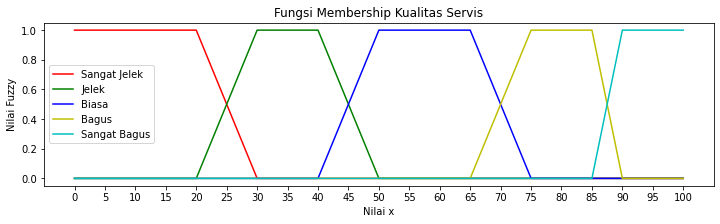
\includegraphics[width=1\linewidth]{images/member_servis.png}
    \caption{Fungsi keanggotaan kualitas servis.}
    \label{fig:member_servis}
\end{figure}


\subsubsection*{Menentukan Fungsi Keanggotaan Harga}
Misalkan nilai harga untuk sebuah bengkel adalah $y$,
maka fungsi keanggotaan (\textit{membership function}) untuk harga didefinisikan secara linguistik sebagai berikut:

\begin{itemize}
    \item Jika $x \leq 3$, maka harga bengkel tersebut diartikan \textbf{murah}.
    \item Jika $5 \leq x \leq 6$, maka harga bengkel tersebut diartikan \textbf{sedang}.
    \item Jika $9 \leq x \leq 10$, maka harga bengkel tersebut diartikan \textbf{mahal}.
\end{itemize}


Sedemikian sehingga, untuk kasus variabel \textbf{harga}, fungsi keanggotaan ditentukan sebagai berikut:

\[
    \mu_{\text{Murah}}(x) =
    \begin{cases}
        1,                    & x \leq 3  \\
        \dfrac{5 - x}{5 - 3}, & 3 < x < 5 \\
        0,                    & x \geq 5
    \end{cases}
\]

\[
    \mu_{\text{Sedang}}(x) =
    \begin{cases}
        0,                    & x \leq 3        \\
        \dfrac{x - 3}{5 - 3}, & 3 < x < 5       \\
        1,                    & 5 \leq x \leq 6 \\
        \dfrac{9 - x}{9 - 6}, & 6 < x < 9       \\
        0,                    & x \geq 9
    \end{cases}
\]

\[
    \mu_{\text{Mahal}}(x) =
    \begin{cases}
        0,                    & x \leq 6  \\
        \dfrac{x - 6}{9 - 6}, & 6 < x < 9 \\
        1,                    & x \geq 9
    \end{cases}
\]

Atau jika digambarkan dalam bentuk grafik, fungsi keanggotaan harga dapat digambarkan sebagaimana pada Gambar \ref{fig:member_harga}.
\begin{figure}[H]
    \centering
    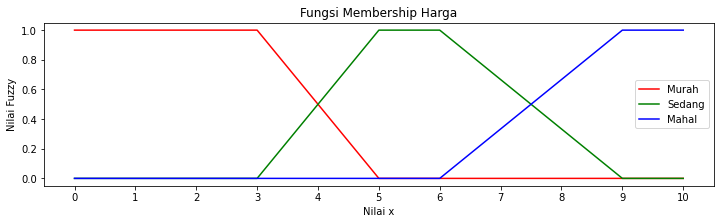
\includegraphics[width=1\linewidth]{images/member_harga.png}
    \caption{Fungsi keanggotaan harga.}
    \label{fig:member_harga}
\end{figure}

\subsubsection*{Menentukan Fuzzifikasi}

Selanjutnya, kita akan menentukan derajat keanggotaan (fuzzifikasi) dari masing-masing data dalam data. Berikut adalah hasil untuk tiga data awal yang dituliskan pada Tabel~\ref{tab:keanggotaan_awal}.

% Kualitas Servis:  58
% Harga:  7
% Nilai Kualitas Servis:  {'Sangat Jelek': 0, 'Jelek': 0, 'Biasa': 1, 'Bagus': 0, 'Sangat Bagus': 0}
% Nilai Harga:  {'Murah': 0, 'Sedang': 0.6666666666666666, 'Mahal': 0.3333333333333333}

% Kualitas Servis:  54
% Harga:  1
% Nilai Kualitas Servis:  {'Sangat Jelek': 0, 'Jelek': 0, 'Biasa': 1, 'Bagus': 0, 'Sangat Bagus': 0}
% Nilai Harga:  {'Murah': 1, 'Sedang': 0, 'Mahal': 0}

% Kualitas Servis:  98
% Harga:  2
% Nilai Kualitas Servis:  {'Sangat Jelek': 0, 'Jelek': 0, 'Biasa': 0, 'Bagus': 0, 'Sangat Bagus': 1}
% Nilai Harga:  {'Murah': 1, 'Sedang': 0, 'Mahal': 0}


\begin{table}[H]
    \centering
    \caption{Derajat Keanggotaan untuk Tiga Data Awal}
    \label{tab:keanggotaan_awal}
    \resizebox{\textwidth}{!}{
        \begin{tabular}{ccccccccccc}
            \toprule
            \multirow{2}{*}{No}                       & \multirow{2}{*}{Kualitas Servis} & \multirow{2}{*}{Harga} &
            \multicolumn{5}{c}{Nilai Kualitas Servis} & \multicolumn{3}{c}{Nilai Harga}                                                                                                          \\
            \cmidrule(lr){4-8} \cmidrule(lr){9-11}
                                                      &                                  &                        & Sangat Jelek & Jelek & Biasa & Bagus & Sangat Bagus & Murah & Sedang & Mahal \\
            \midrule
            1                                         & 58                               & 7                      & 0            & 0     & 1     & 0     & 0            & 0     & 0.667  & 0.333 \\
            2                                         & 54                               & 1                      & 0            & 0     & 1     & 0     & 0            & 1     & 0      & 0     \\
            3                                         & 98                               & 2                      & 0            & 0     & 0     & 0     & 1            & 1     & 0      & 0     \\
            \bottomrule
        \end{tabular}
    }
\end{table}

\subsubsection*{Menentukan Aturan Inferensi}

Setelah mendapatkan hasil fuzzifikasi dari masing-masing data, selanjutnya kita akan menentukan aturan inferensi dalam sistem fuzzy ini. Aturan inferensi fuzzy ditentukan sebagaimana dalam Tabel~\ref{tab:aturan_inferensi}.

\begin{table}[H]
    \centering
    \caption{Aturan Inferensi Fuzzy Berdasarkan Harga dan Kualitas Servis}
    \label{tab:aturan_inferensi}
    \resizebox{\linewidth}{!}{
        \begin{tabular}{lccccc}
            \toprule
            \multirow{2}{*}{Harga} & \multicolumn{5}{c}{Kualitas Servis}                                                                                                 \\
            \cmidrule(lr){2-6}
                                   & Sangat Jelek                        & Jelek                  & Biasa            & Bagus                   & Sangat Bagus            \\
            \midrule
            Murah                  & Tidak Direkomendasikan              & Tidak Direkomendasikan & Direkomendasikan & Sangat Direkomendasikan & Sangat Direkomendasikan \\
            Sedang                 & Tidak Direkomendasikan              & Tidak Direkomendasikan & Alternatif       & Direkomendasikan        & Sangat Direkomendasikan \\
            Mahal                  & Tidak Direkomendasikan              & Tidak Direkomendasikan & Alternatif       & Direkomendasikan        & Direkomendasikan        \\
            \bottomrule
        \end{tabular}
    }
\end{table}

Setiap aturan pada Tabel~\ref{tab:aturan_inferensi} diartikan sebagai \textit{aturan konjungsi}. Sebagai contoh, diperoleh

\[
    \text{IF } (\text{Harga} = \text{Murah})(1) \land (\text{Servis} = \text{Sangat Jelek})(1) \text{ THEN } (\text{Status} = \text{Tidak Direkomendasikan}(1))
\]

dengan hasil inferensi $Status=\textit{Tidak Direkomendasikan(1)}$, "Tidak Direkomendasikan" didapatkan dari aturan pada Tabel~\ref{tab:aturan_inferensi}, sementara nilai (1), didapatkan dari aturan konjungsi pada Persamaan~\ref{eq:konjungsi_minimum}.

\subsubsection*{Menentukan Defuzzifikasi}

Setelah itu, kita menentukan metode defuzzifikasi yang akan digunakan. Misal, kita menggunakan metode Sugeno model singleton. Kita menentukan batas nilai untuk tiap status, dan didapatkan Gambar~\ref{fig:model_sugeno} sebagai berikut.

\begin{figure}[H]
    \centering
    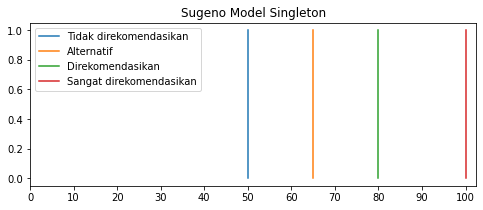
\includegraphics[width=1\linewidth]{images/hasil_sugeno.png}
    \caption{Sugeno model singleton.}
    \label{fig:model_sugeno}
\end{figure}

Untuk masing-masing nilai pada data, dengan menggunakan Persamaan~\ref{eq:defuzzifikasi_sugeno}, didapatkan hasil berikut.

% Data Ke-1 = 65.0
% Data Ke-2 = 80.0
% Data Ke-3 = 100.0
\begin{table}[H]
    \centering
    \caption{Hasil defuzzifikasi untuk tiga data awal}
    \label{tab:hasil_defuzzifikasi}
    \begin{tabular}{|c|c|}
        \hline
        \textbf{id} & \textbf{Hasil defuzzifikasi} \\ \hline
        1           & 65                           \\
        2           & 80                           \\
        3           & 100                          \\
        \hline
    \end{tabular}
\end{table}

\subsubsection*{Mendapatkan tiga bengkel terbaik}

Setelah itu, misal kita ingin mendapatkan tiga bengkel yang terbaik, kita tinggal mengurutkan berdasarkan hasilnya, dan didapatkanlah hasil pada Tabel~\ref{tab:hasil_terbaik} berikut.

% 	id	servis	harga	result
% 2	3	98	2	100.0
% 51	52	94	3	100.0
% 33	34	93	4	100.0
% 91	92	83	3	100.0

\begin{table}[H]
    \centering
    \caption{Daftar Servis dan Harga Bengkel}
    \label{tab:hasil_terbaik}
    \begin{tabular}{|c|c|c|c|}
        \hline
        \textbf{id} & \textbf{servis} & \textbf{harga} & \textbf{hasil} \\ \hline
        3           & 98              & 2              & 100            \\
        52          & 94              & 3              & 100            \\
        34          & 93              & 4              & 100            \\
        \hline
    \end{tabular}
\end{table}

% \begin{figure}
%     \centering
%     \includegraphics[width=0.5\linewidth]{}
%     \caption{Caption}
%     \label{fig:placeholder}
% \end{figure}

\section{Coding Penyelesaian Masalah}
\subsection*{Menentukan fungsi keanggotaan}
\subsubsection*{Kualitas servis}
\begin{verbatim}
# fungsi membership kualitas servis
def membershipKualitasServis(x):
  kualitasServis = {"Sangat Jelek": 0, "Jelek": 0,"Biasa": 0,
  "Bagus": 0,"Sangat Bagus": 0}

  a,b,c,d,e,f,g,h,i = 20,30,40,50,65,75,85,90,100

  # garis datar
  if x <= a:
    kualitasServis["Sangat Jelek"] = 1
  if x >= b and x <= c:
    kualitasServis["Jelek"] = 1
  if x >= d and x <= e:
    kualitasServis["Biasa"] = 1
  if x >= f and x <= g:
    kualitasServis["Bagus"] = 1
  if x >= h and x <= i:
    kualitasServis["Sangat Bagus"] = 1

  # garis miring
  if x > a and x <= b:
    kualitasServis["Sangat Jelek"] = -(x - b) / (b - a)
  if x > a and x < b:
    kualitasServis["Jelek"] = (x - a) / (b - a)
  if x > c and x <= d:
    kualitasServis["Jelek"] = -(x - d) / (d - c)
  if x > c and x < d:
    kualitasServis["Biasa"] = (x - c) / (d - c)  
  if x > e and x <= f:
    kualitasServis["Biasa"] = -(x - f) / (f - e)
  if x > e and x < f:
    kualitasServis["Bagus"] = (x - e) / (f - e) 
  if x > g and x <= h:
    kualitasServis["Bagus"] = -(x - h) / (h - g)
  if x > g and x < h:
    kualitasServis["Sangat Bagus"] = (x - g) / (h - g) 
  
  return kualitasServis

# Diagram nilai kualitas servis
plt.figure(figsize=(12,3))
plt.title("Fungsi Membership Kualitas Servis")

plt.plot(range(101),[membershipKualitasServis(x)["Sangat Jelek"] 
for x in range(101)], "r")
plt.plot(range(101),[membershipKualitasServis(x)["Jelek"] 
for x in range(101)], "g")
plt.plot(range(101),[membershipKualitasServis(x)["Biasa"] 
for x in range(101)], "b")
plt.plot(range(101),[membershipKualitasServis(x)["Bagus"] 
for x in range(101)], "y")
plt.plot(range(101),[membershipKualitasServis(x)["Sangat Bagus"] 
for x in range(101)], "c")

plt.plot(0, 0, "r", linewidth = 1.5, label = "Sangat Jelek")
plt.plot(0, 0, "g", linewidth = 1.5, label = "Jelek")
plt.plot(0, 0, "b", linewidth = 1.5, label = "Biasa")
plt.plot(0, 0, "y", linewidth = 1.5, label = "Bagus")
plt.plot(0, 0, "c", linewidth = 1.5, label = "Sangat Bagus")

plt.xticks(np.arange(0, 105, 5.0))
plt.xlabel("Nilai x")
plt.ylabel("Nilai Fuzzy")
plt.legend()
plt.show()
\end{verbatim}
\subsubsection*{Harga}
\begin{verbatim}
# fungsi membership harga
def membershipHarga(x):
  harga = {"Murah": 0,"Sedang": 0,"Mahal": 0}

  a,b,c,d,e = 3,5,6,9,10

  # garis datar
  if x <= a:
    harga["Murah"] = 1
  if x >= b and x <= c:
    harga["Sedang"] = 1
  if x >= d and x <= e:
    harga["Mahal"] = 1

  # garis miring
  if x > a and x <= b:
    harga["Murah"] = -(x - b) / (b - a)
  if x > a and x < b:
    harga["Sedang"] = (x - a) / (b - a)
  if x > c and x <= d:
    harga["Sedang"] = -(x - d) / (d - c)
  if x > c and x < d:
    harga["Mahal"] = (x - c) / (d - c)  
  
  return harga

# Diagram nilai harga
plt.figure(figsize=(12,3))
plt.title("Fungsi Membership Harga")

plt.plot(range(11),[membershipHarga(x)["Murah"] for x in range(11)], "r")
plt.plot(range(11),[membershipHarga(x)["Sedang"] 
for x in range(11)], "g")
plt.plot(range(11),[membershipHarga(x)["Mahal"] for x in range(11)], "b")

plt.plot(0, 0, "r", linewidth = 1.5, label = "Murah")
plt.plot(0, 0, "g", linewidth = 1.5, label = "Sedang")
plt.plot(0, 0, "b", linewidth = 1.5, label = "Mahal")

plt.xticks(list(range(11)))
plt.xlabel("Nilai x")
plt.ylabel("Nilai Fuzzy")
plt.legend()
plt.show()

\end{verbatim}
\subsection*{Menentukan hasil fuzzifikasi}
\begin{verbatim}
kumpulanNilaiFuzzy = []

for kualitasServis, harga in zip(bengkel["servis"], bengkel['harga']):
  nilaiFuzzy = {"Kualitas Servis ": 0, "Harga": 0, 
  "Nilai Fuzzy Kualitas Servis": 0, "Nilai Fuzzy Harga": 0}

  nilaiFuzzy["Kualitas Servis"] = kualitasServis
  nilaiFuzzy["Harga"] = harga
  nilaiFuzzy["Nilai Fuzzy Kualitas Servis"] = 
  membershipKualitasServis(kualitasServis)
  nilaiFuzzy["Nilai Fuzzy Harga"] = membershipHarga(harga)

  kumpulanNilaiFuzzy.append(nilaiFuzzy)
\end{verbatim}
\subsection*{Menentukan aturan inferensi}
\begin{verbatim}
#Untuk setiap rules merupakan Konjungsi.
#Contoh: IF Harga = Murah (1) ^ Servis = Sangat Jelek (1) THEN Status = Tidak Direkomendasikan

fuzzySetRules = {
    ('Murah', 'Sangat Jelek') : 'Tidak Direkomendasikan',
    ('Sedang', 'Sangat Jelek') : 'Tidak Direkomendasikan',
    ('Mahal', 'Sangat Jelek'): 'Tidak Direkomendasikan',
    ('Murah', 'Jelek'): 'Tidak Direkomendasikan',
    ('Sedang', 'Jelek'): 'Tidak Direkomendasikan',
    ('Mahal', 'Jelek'): 'Tidak Direkomendasikan',
    ('Murah', 'Biasa'): 'Direkomendasikan',
    ('Sedang', 'Biasa'): 'Alternatif',
    ('Mahal', 'Biasa'): 'Alternatif',
    ('Murah', 'Bagus'): 'Sangat Direkomendasikan',
    ('Sedang', 'Bagus'): 'Direkomendasikan',
    ('Mahal', 'Bagus'): 'Direkomendasikan',
    ('Murah', 'Sangat Bagus'): 'Sangat Direkomendasikan',
    ('Sedang', 'Sangat Bagus'): 'Sangat Direkomendasikan',
    ('Mahal', 'Sangat Bagus'): 'Direkomendasikan',
}
\end{verbatim}
\subsection*{Menentukan hasil inferensi}
\begin{verbatim}
hasilInterefence = []

def interefence(fuzzed):
    result = {'Nilai Fuzzy':0, 'Tidak Direkomendasikan': 0, 
    'Alternatif': 0, 'Direkomendasikan': 0, 'Sangat Direkomendasikan': 0}

    for Servis in fuzzed['Nilai Fuzzy Kualitas Servis'].keys():
        for Harga in fuzzed['Nilai Fuzzy Harga'].keys():
            result["Nilai Fuzzy"] = 
            {"Kualitas Servis": fuzzed["Kualitas Servis"], 
            "Harga": fuzzed["Harga"]}
            minValue = min(fuzzed['Nilai Fuzzy Harga'][Harga], 
            fuzzed['Nilai Fuzzy Kualitas Servis'][Servis])

            #Proses Konjungsi sesuai fuzzy set rules
            output = fuzzySetRules[(Harga, Servis)]

            if minValue > result[output]:
                result[output] = minValue

    return result

for fuzzed in kumpulanNilaiFuzzy:
    hasilInterefence.append(interefence(fuzzed))
\end{verbatim}
\subsubsection*{Menentukan defuzzifikasi}
\begin{verbatim}
deffuzy = {'Tidak Direkomendasikan': 50, "Alternatif": 65, "Direkomendasikan": 80, "Sangat Direkomendasikan": 100}

def defuzzification(inference, deffuzy):
    numerator, denominator = 0, 0
    
    for output in deffuzy.keys():
        numerator += inference[output] * deffuzy[output]
        denominator += inference[output]
        
    return numerator/denominator

hasilAkhir = []

for inference in hasilInterefence:
    hasilAkhir.append(defuzzification(inference, deffuzy))
\end{verbatim}
\subsection*{Menampilkan hasil terbaik}
\begin{verbatim}
bengkel['result'] = hasilAkhir
bengkel = bengkel.sort_values(by='result', ascending=False)[:10]

bengkel['id'].to_excel('peringkat.xls', index=False, header=False)  
bengkel
\end{verbatim}

Dataset yang digunakan dan Kode dalam tugas ini telah diunggah di Repository github pada pranala berikut \url{https://github.com/khalilullahalfaath/Materi-Fuzzy-Logic/blob/main/tutorials}.

\section{Hasil dan Interpretasinya}

% \subsubsection*{Mendapatkan Tiga Bengkel Terbaik}

Setelah seluruh data bengkel diproses melalui tahapan fuzzifikasi, inferensi, dan defuzzifikasi, setiap bengkel memperoleh nilai akhir yang merepresentasikan tingkat rekomendasi berdasarkan kombinasi antara \textit{kualitas servis} dan \textit{harga}. Nilai ini menunjukkan seberapa layak suatu bengkel direkomendasikan kepada pengguna.

Langkah selanjutnya adalah melakukan pengurutan terhadap seluruh nilai hasil inferensi untuk mengidentifikasi bengkel dengan performa tertinggi. Dari proses pengurutan tersebut, diperoleh tiga bengkel dengan nilai hasil akhir tertinggi, yaitu sebesar 100. Nilai ini menunjukkan bahwa ketiga bengkel tersebut memenuhi kriteria maksimum pada fungsi keanggotaan fuzzy untuk kategori \textit{Sangat Direkomendasikan}. Hasilnya dapat dilihat pada Tabel~\ref{tab:hasil_terbaik_kesimpulan}.

\begin{table}[H]
    \centering
    \caption{Daftar Servis dan Harga Bengkel Terbaik}
    \label{tab:hasil_terbaik_kesimpulan}
    \begin{tabular}{|c|c|c|c|}
        \hline
        \textbf{id} & \textbf{Kualitas Servis} & \textbf{Harga} & \textbf{Hasil Akhir} \\ \hline
        3           & 98                       & 2              & 100                  \\
        52          & 94                       & 3              & 100                  \\
        34          & 93                       & 4              & 100                  \\
        \hline
    \end{tabular}
\end{table}

Ketiga bengkel tersebut memiliki nilai \textit{kualitas servis} yang sangat tinggi (di atas 90) serta harga yang relatif rendah. Kombinasi ini menghasilkan tingkat rekomendasi maksimal karena sesuai dengan aturan inferensi fuzzy pada Tabel~\ref{tab:aturan_inferensi}, di mana kondisi \textit{Servis = Sangat Bagus} dan \textit{Harga = Murah atau Sedang} memberikan output \textit{Status = Sangat Direkomendasikan}. Dengan demikian, sistem berhasil mengidentifikasi bahwa bengkel dengan kualitas servis tinggi dan harga kompetitif merupakan pilihan terbaik bagi pengguna.

Secara interpretatif, hasil ini memperkuat validitas sistem fuzzy yang dibangun. Sistem mampu menyeimbangkan antara dua faktor utama, yaitu kualitas dan harga, secara adaptif tanpa memerlukan batasan kaku seperti pada metode deterministik. Nilai hasil akhir 100 menunjukkan bahwa aturan konjungsi fuzzy menghasilkan tingkat keanggotaan penuh pada kategori rekomendasi tertinggi.


% \section{Referensi}
\newpage
\printbibliography[title={Referensi}]

\end{document}
